\section{Presentation Logic Layer}

%What pages will be present in your project? briefly indicate how your web site will be organized



The web site have two main sections: Game section and Player section.\\
The pages developed for the Lupus in Fabula web app are as follows:
\begin{itemize}
    \item \textbf{Login/Signup Page:} Single page use for both login and sign up, allowing each user to have his own account, where the games he plays will be saved
    \item \textbf{Home page:} Allows to access the personal area, to enter in an existing game or create a new one and view their logs and statistics.
    \item \textbf{Rules page:} On this page, users can view the game is rules and the various roles.
    \item \textbf{Game section:} in this section the player can create a game and take the role of game-master or if the user is already inside a game in progress it allows him to view his role.
    \begin{itemize}
        \item \textbf{Game settings page:} on this page, if the player is not already in a game, it will allow him to create a new one, otherwise he can enter the current game.
        \item \textbf{InGame Master view page:} page dedicated only to the game-master, it is similar to the Player page, but from this page the game-master can not only see the status of the game, but also which player has which role. Furthermore, he can mark the actions that the players perform.
        \item \textbf{InGame Player view page:} this page is dedicated to players who are participating in a game, they can see their role and current game status (e.g. who is alive and who is dead)
        \item \textbf{Log page:} shows the actions that happened during the game.
    \end{itemize}
    \item \textbf{Player section} In this section the player can view his statistics, e.g. how long he has been playing, how many games he has won, etc., and can see the history of the games he has played.
    \begin{itemize}
        \item \textbf{User page:} From here the user can see his or her own information, e.g. email, change password and manage friends.
        \item \textbf{Statistics and Logs page:} the user can see the statistics of the matches he has played, e.g. the number of matches played, won and lost, roles most played etc, and shows the logs of the games that he played
    \end{itemize}
\end{itemize}

%For the main pages put a mockup and describe it in detail.
\subsection{Login/Signup page}
\begin{figure}[h!] 
    \centering
    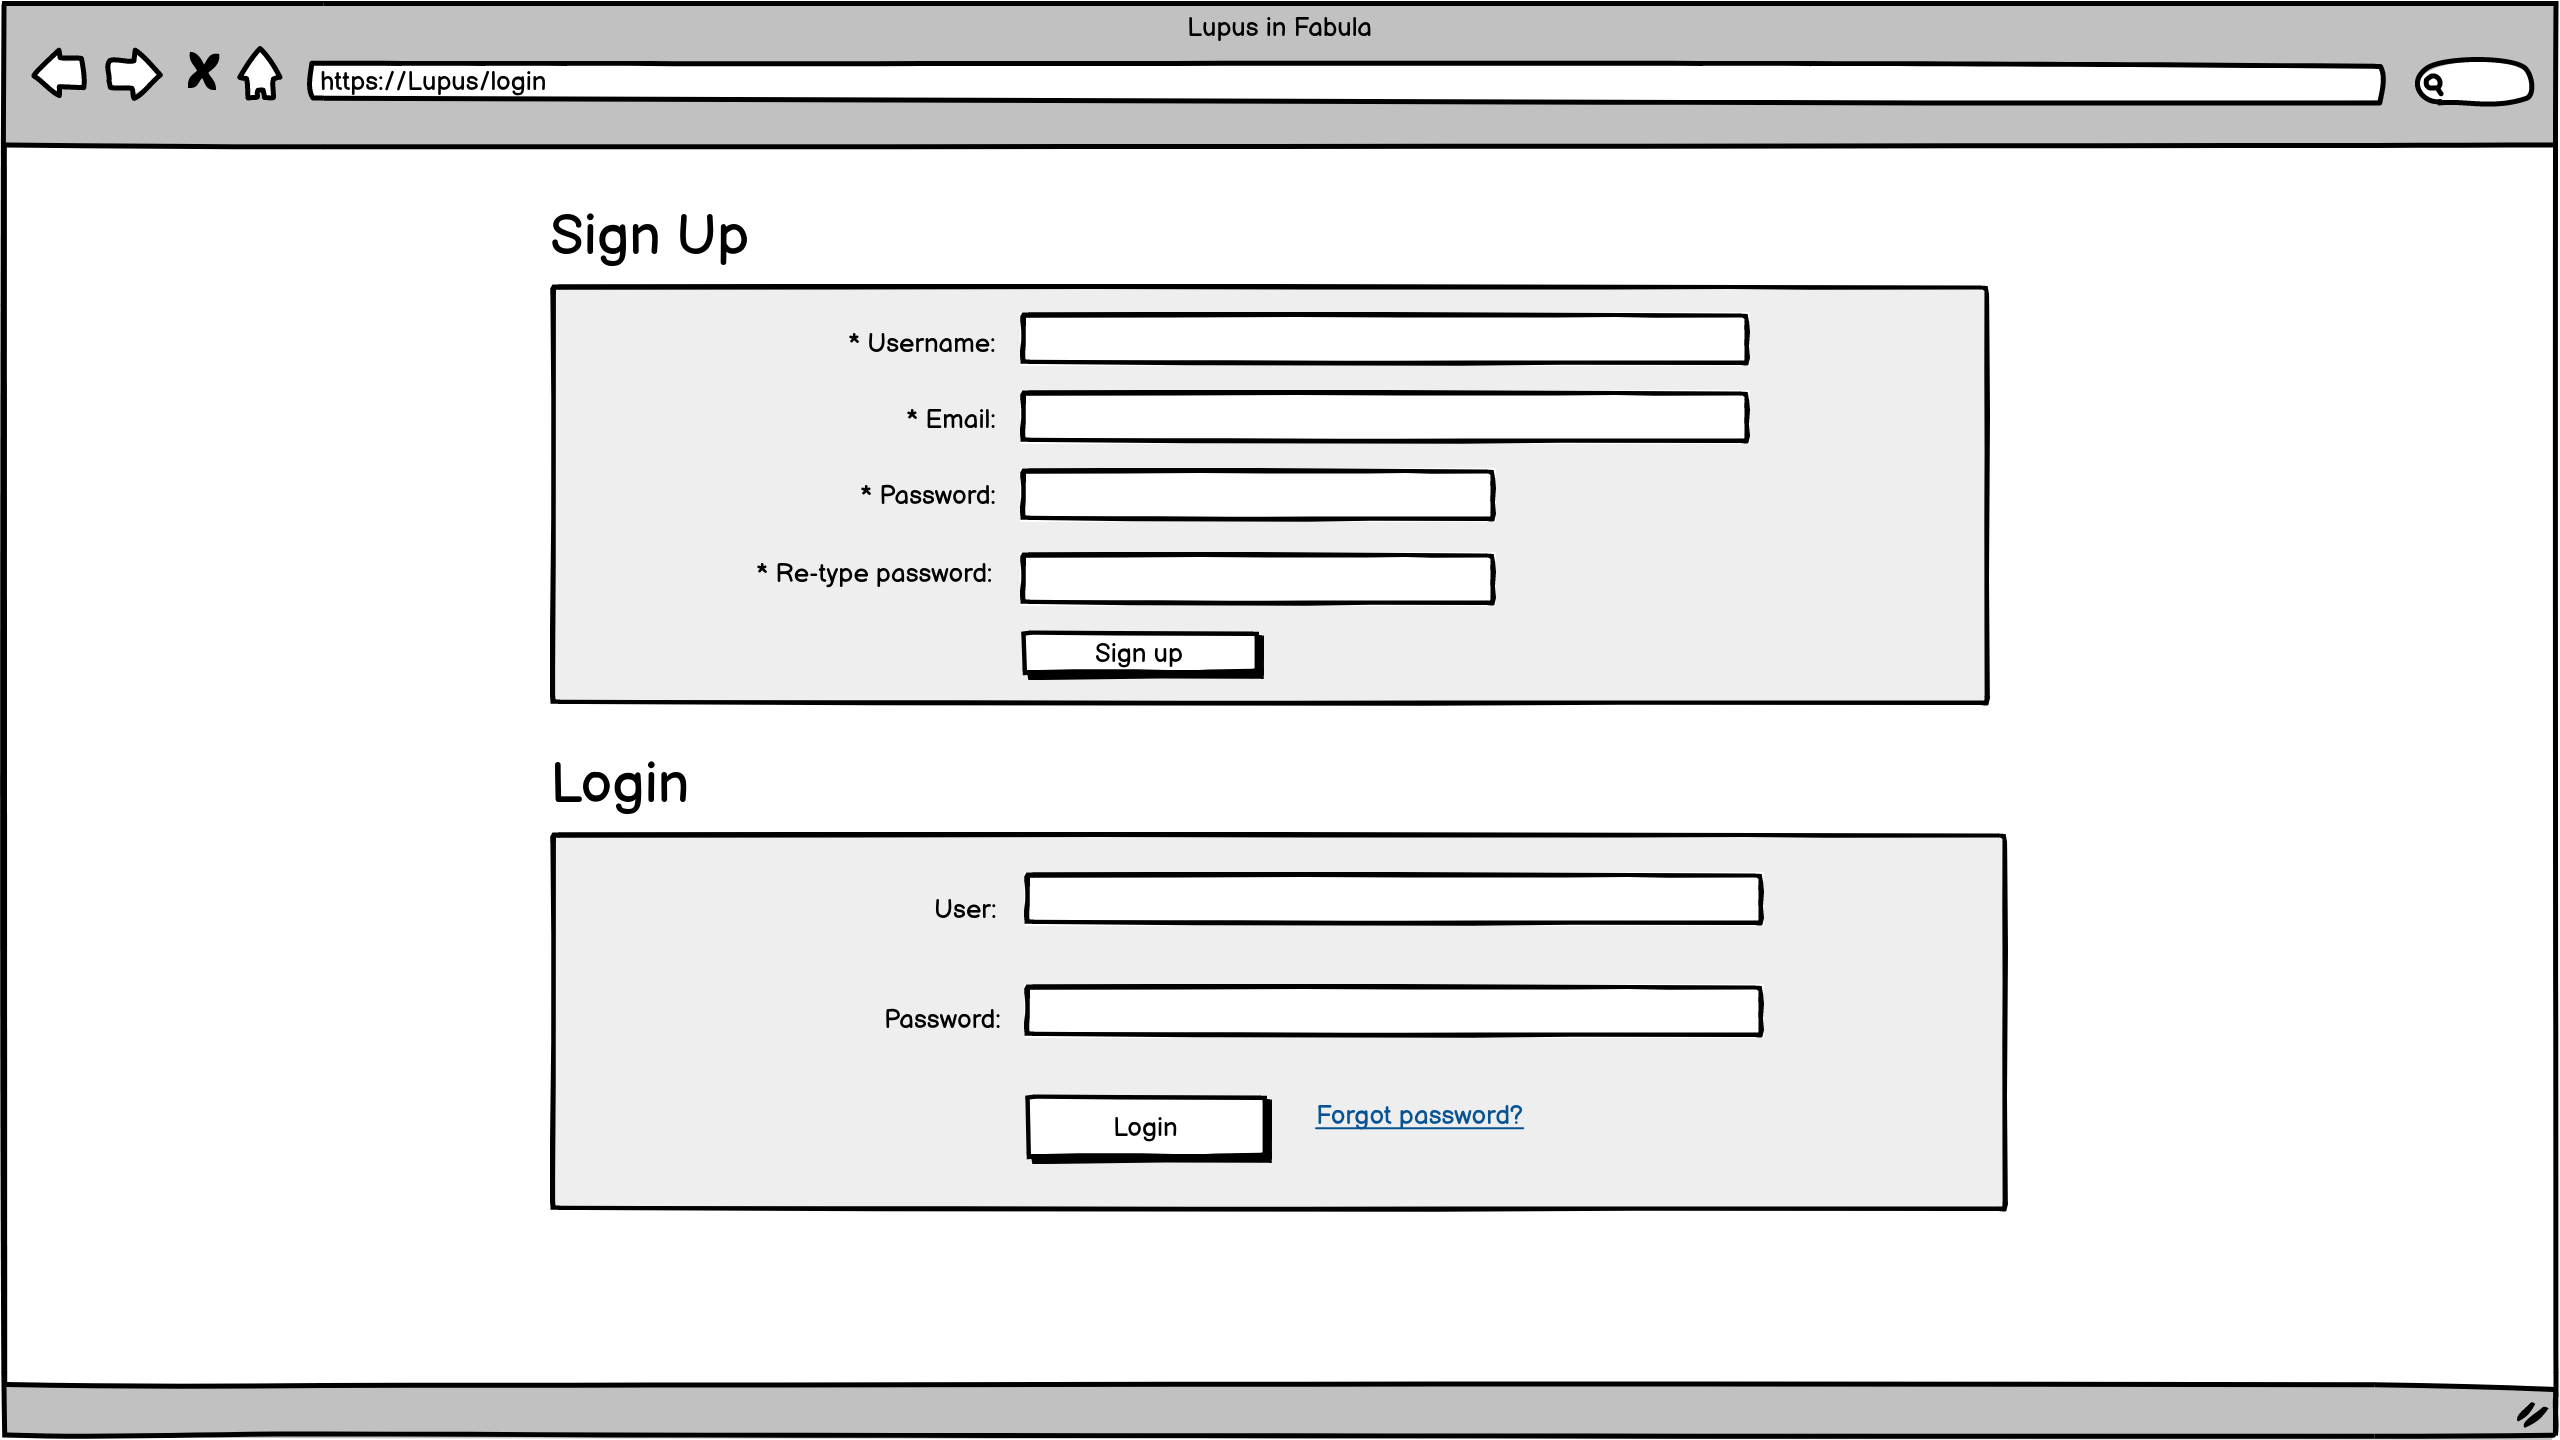
\includegraphics[height=6cm]{images/Page/Login_singup.png}
    \caption{Login/Signup page}
    \label{fig:Login_singup_page}
\end{figure}

We have a single page that allows the user to login or sign up into the system.
For the sign up we require an unique username and email. To do the login it's possible to use either, a username or the email, combined with the password.
A data check is carried out, e.g. the username's length must be between 3 and 29 characters, the email must be of a correct format and the password must comply with security standards, i.e. be 8 characters, with upper, lower case, numbers and special characters, (see figure \ref{fig:Login_singup_page}).

\subsection{Home page (Interface Mockup)}
\begin{figure}[h!] 
    \centering
    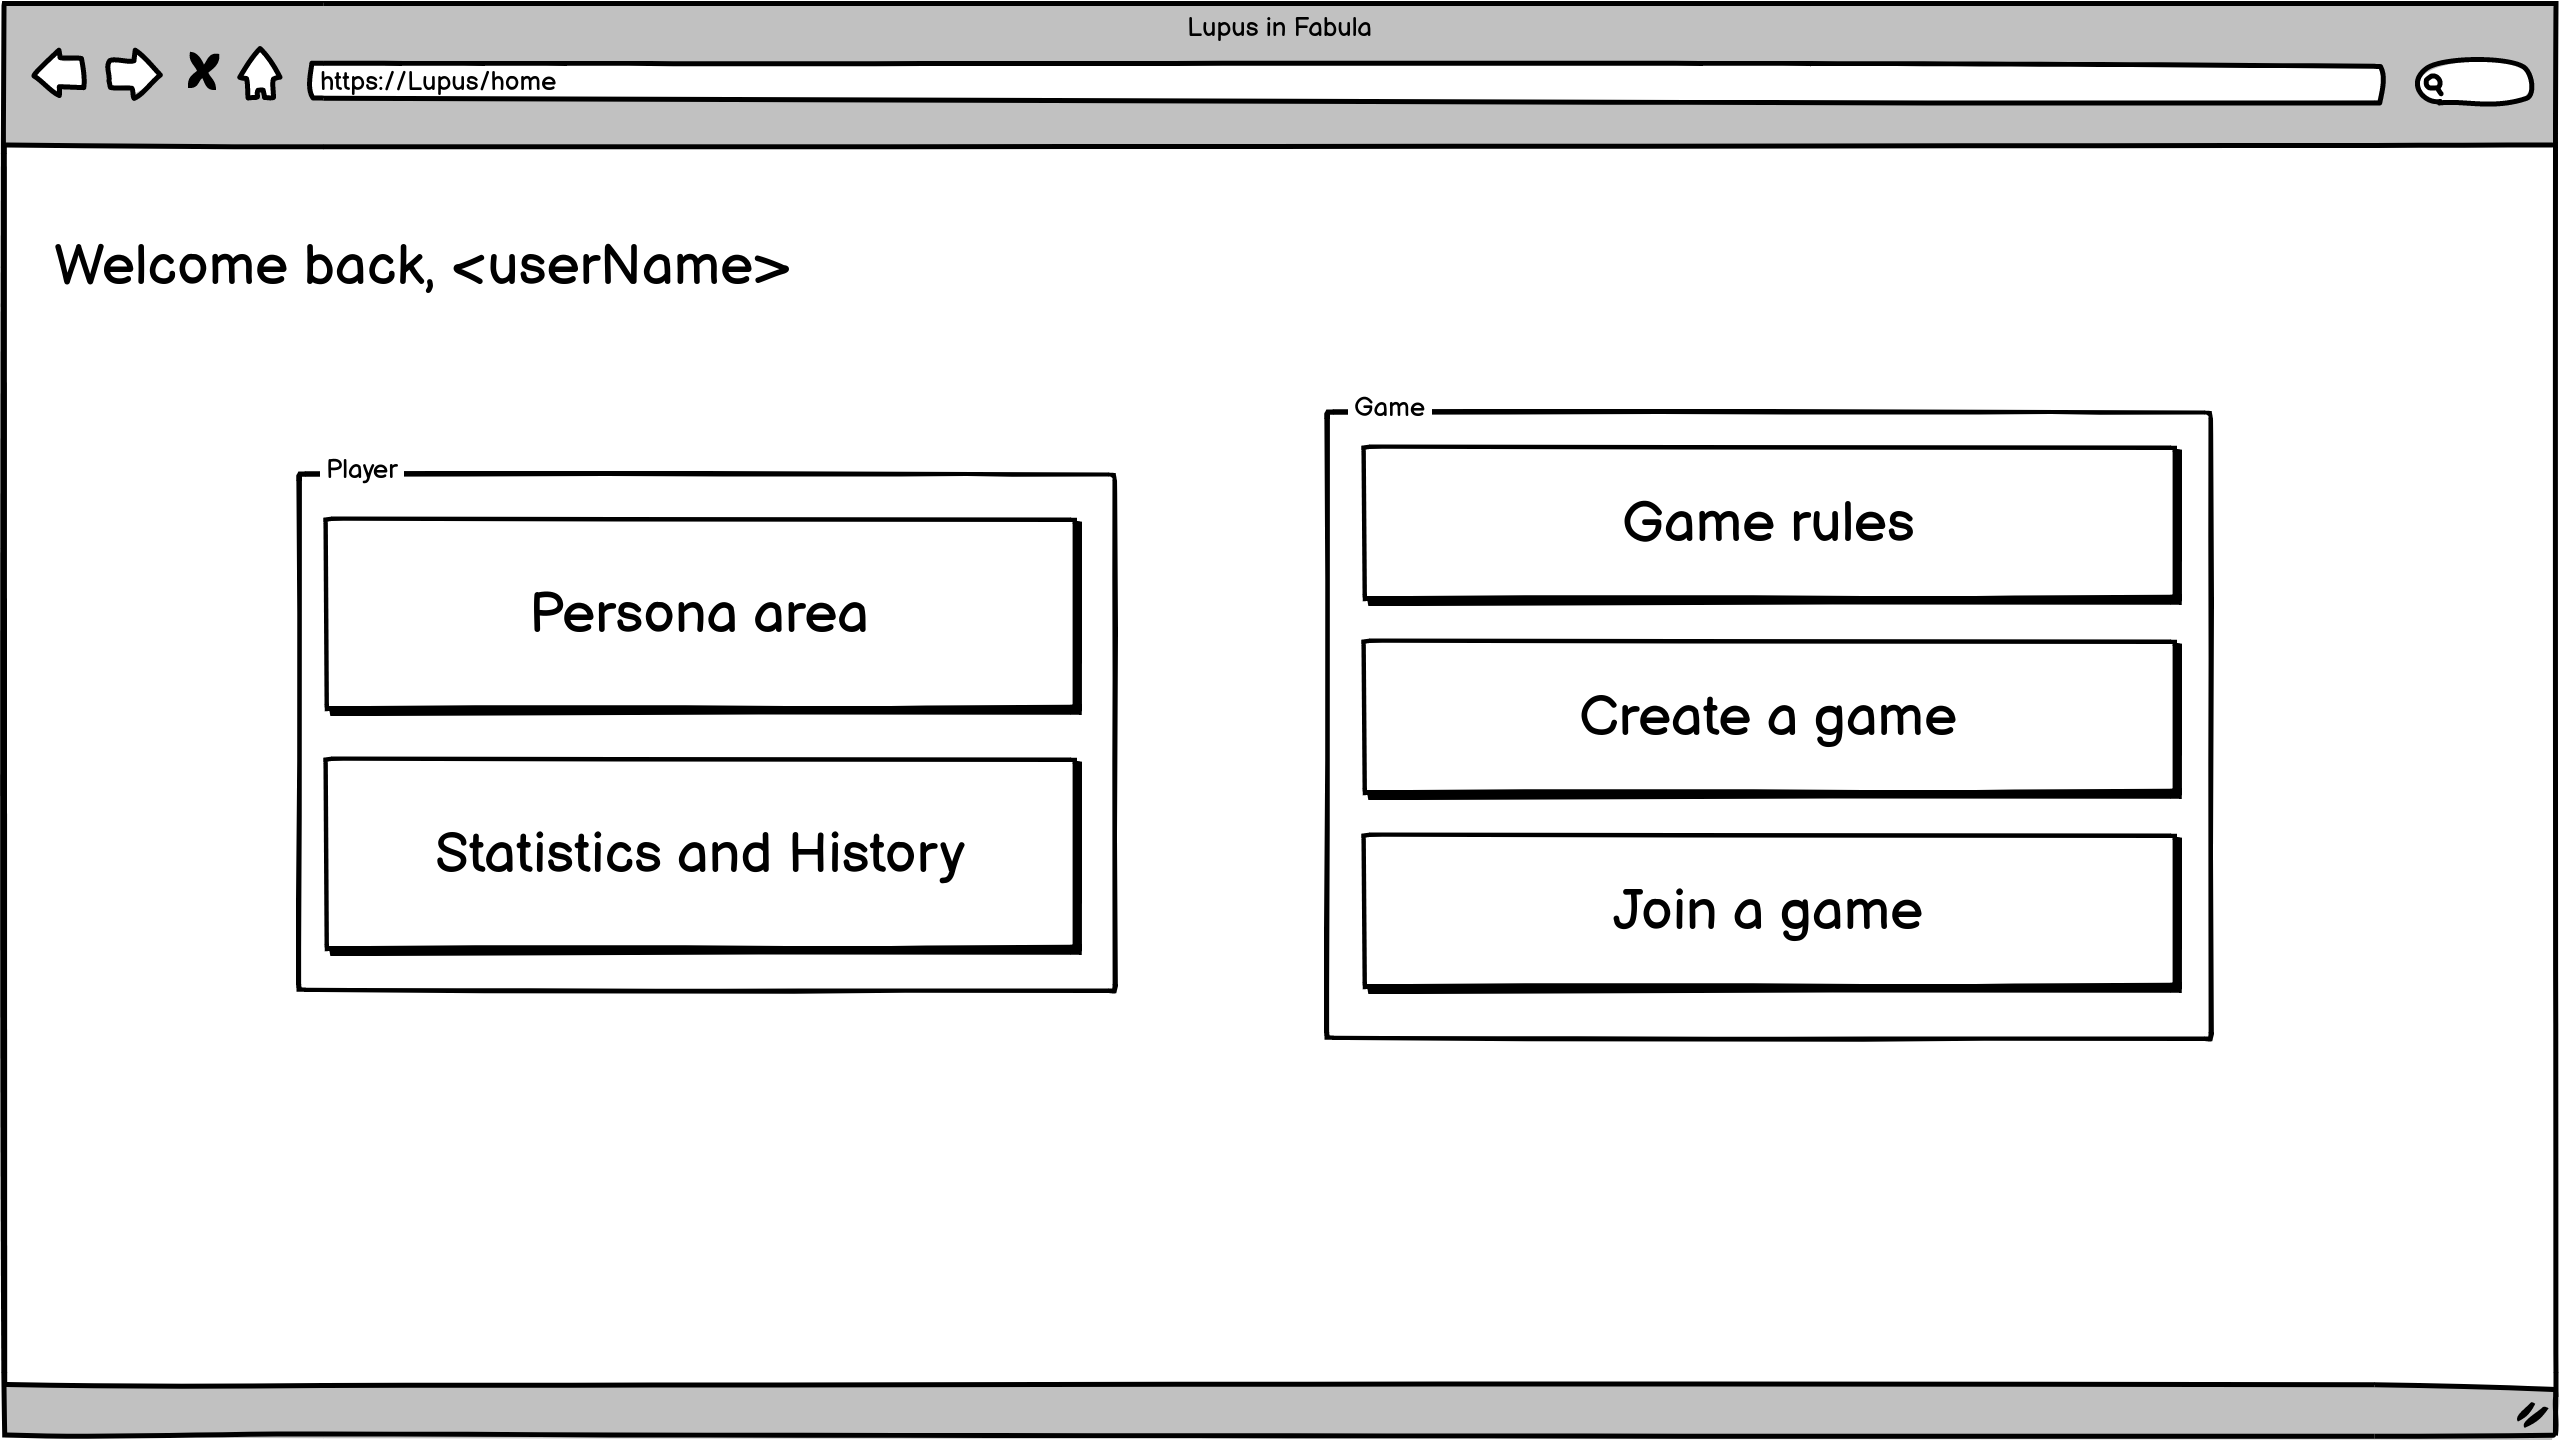
\includegraphics[height=6cm]{images/Page/Home.png}
    \caption{Home page}
    \label{fig:home_page}

\end{figure}

From here, the user can access the main sections of the site, i.e. he can create a game (but only if he is not already in a game that he has started), enter a game in which he is a playing player, access his statistics and see his game history, or he can enter his private area, (see figure \ref{fig:home_page}).

\subsection{Rules page (Interface Mockup)}

\begin{figure}[htb] 
    \centering
    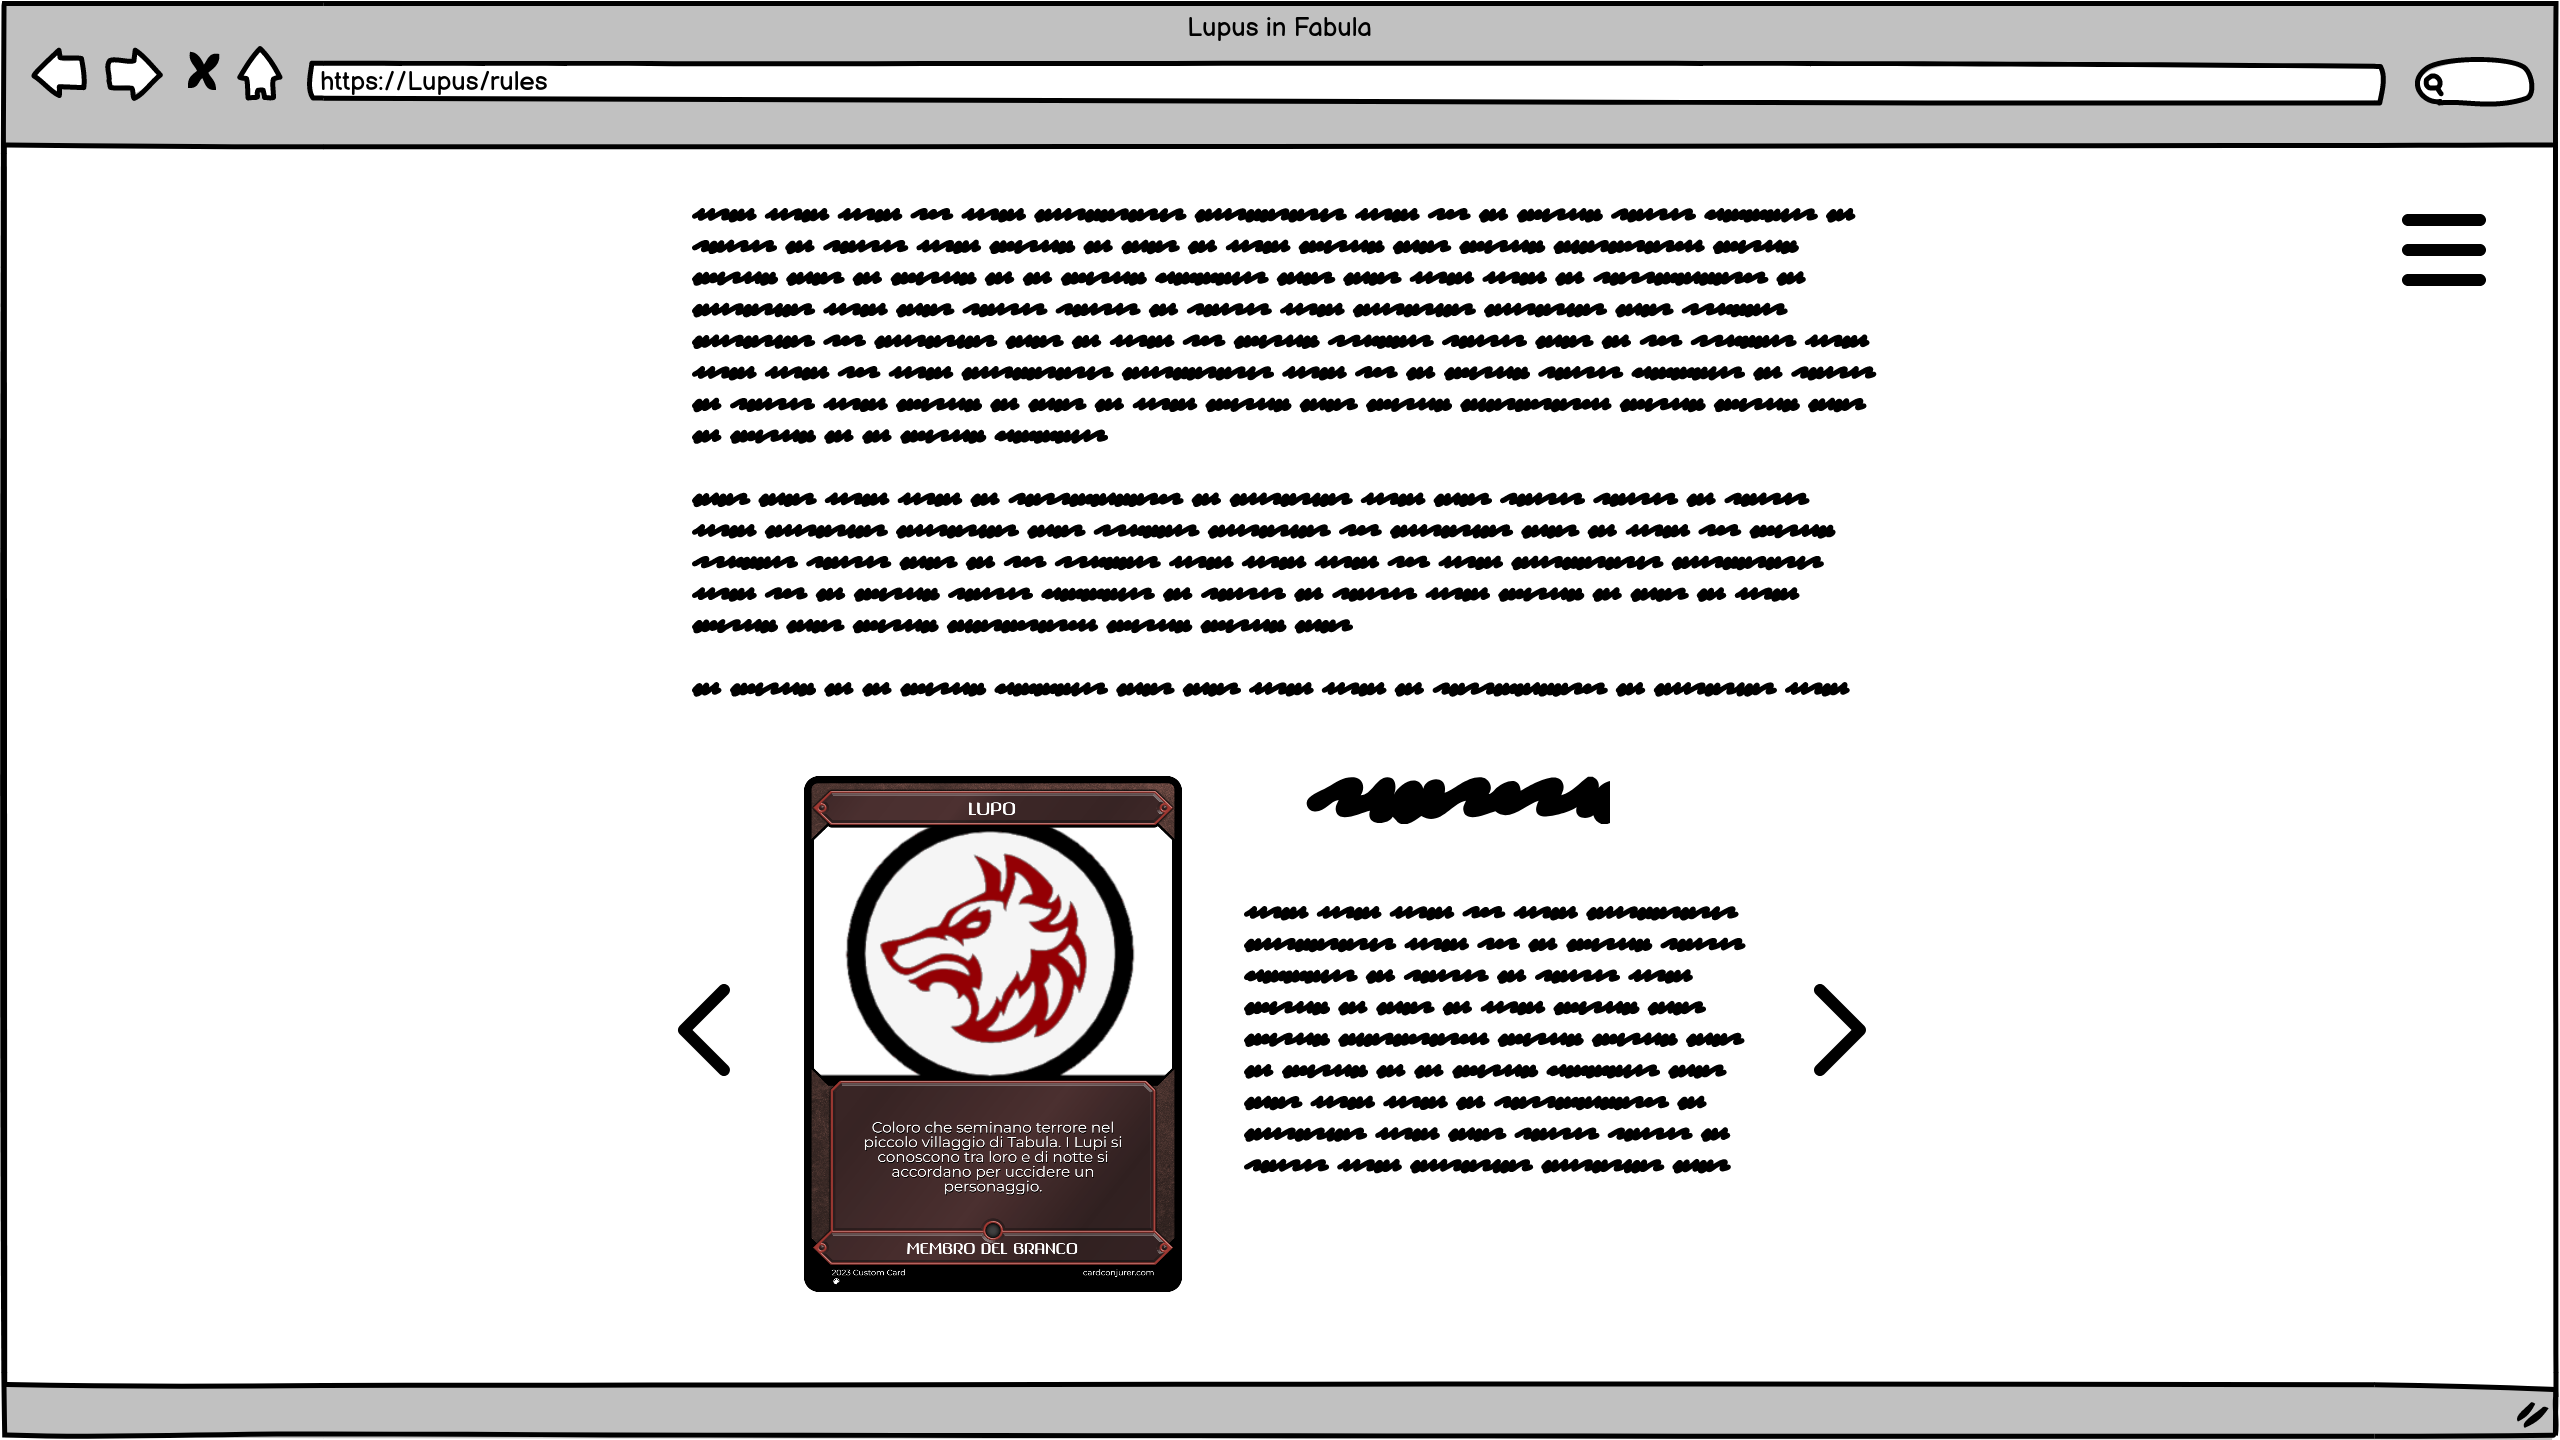
\includegraphics[height=6cm]{images/Page/Rules.png}
    \caption{Rules page}
    \label{fig:rules_page}
\end{figure}
On this page it is possible to see all the rules of the game,  so what Lupus in Fabula is and how to play it, and it also shows the roles in the game, with their characteristics and how they win, divided into various categories, (see figure \ref{fig:rules_page}).

\subsection{Game section}

\subsubsection{Game settings page (Interface Mockup)}
\begin{figure}[htb] 
    \centering
    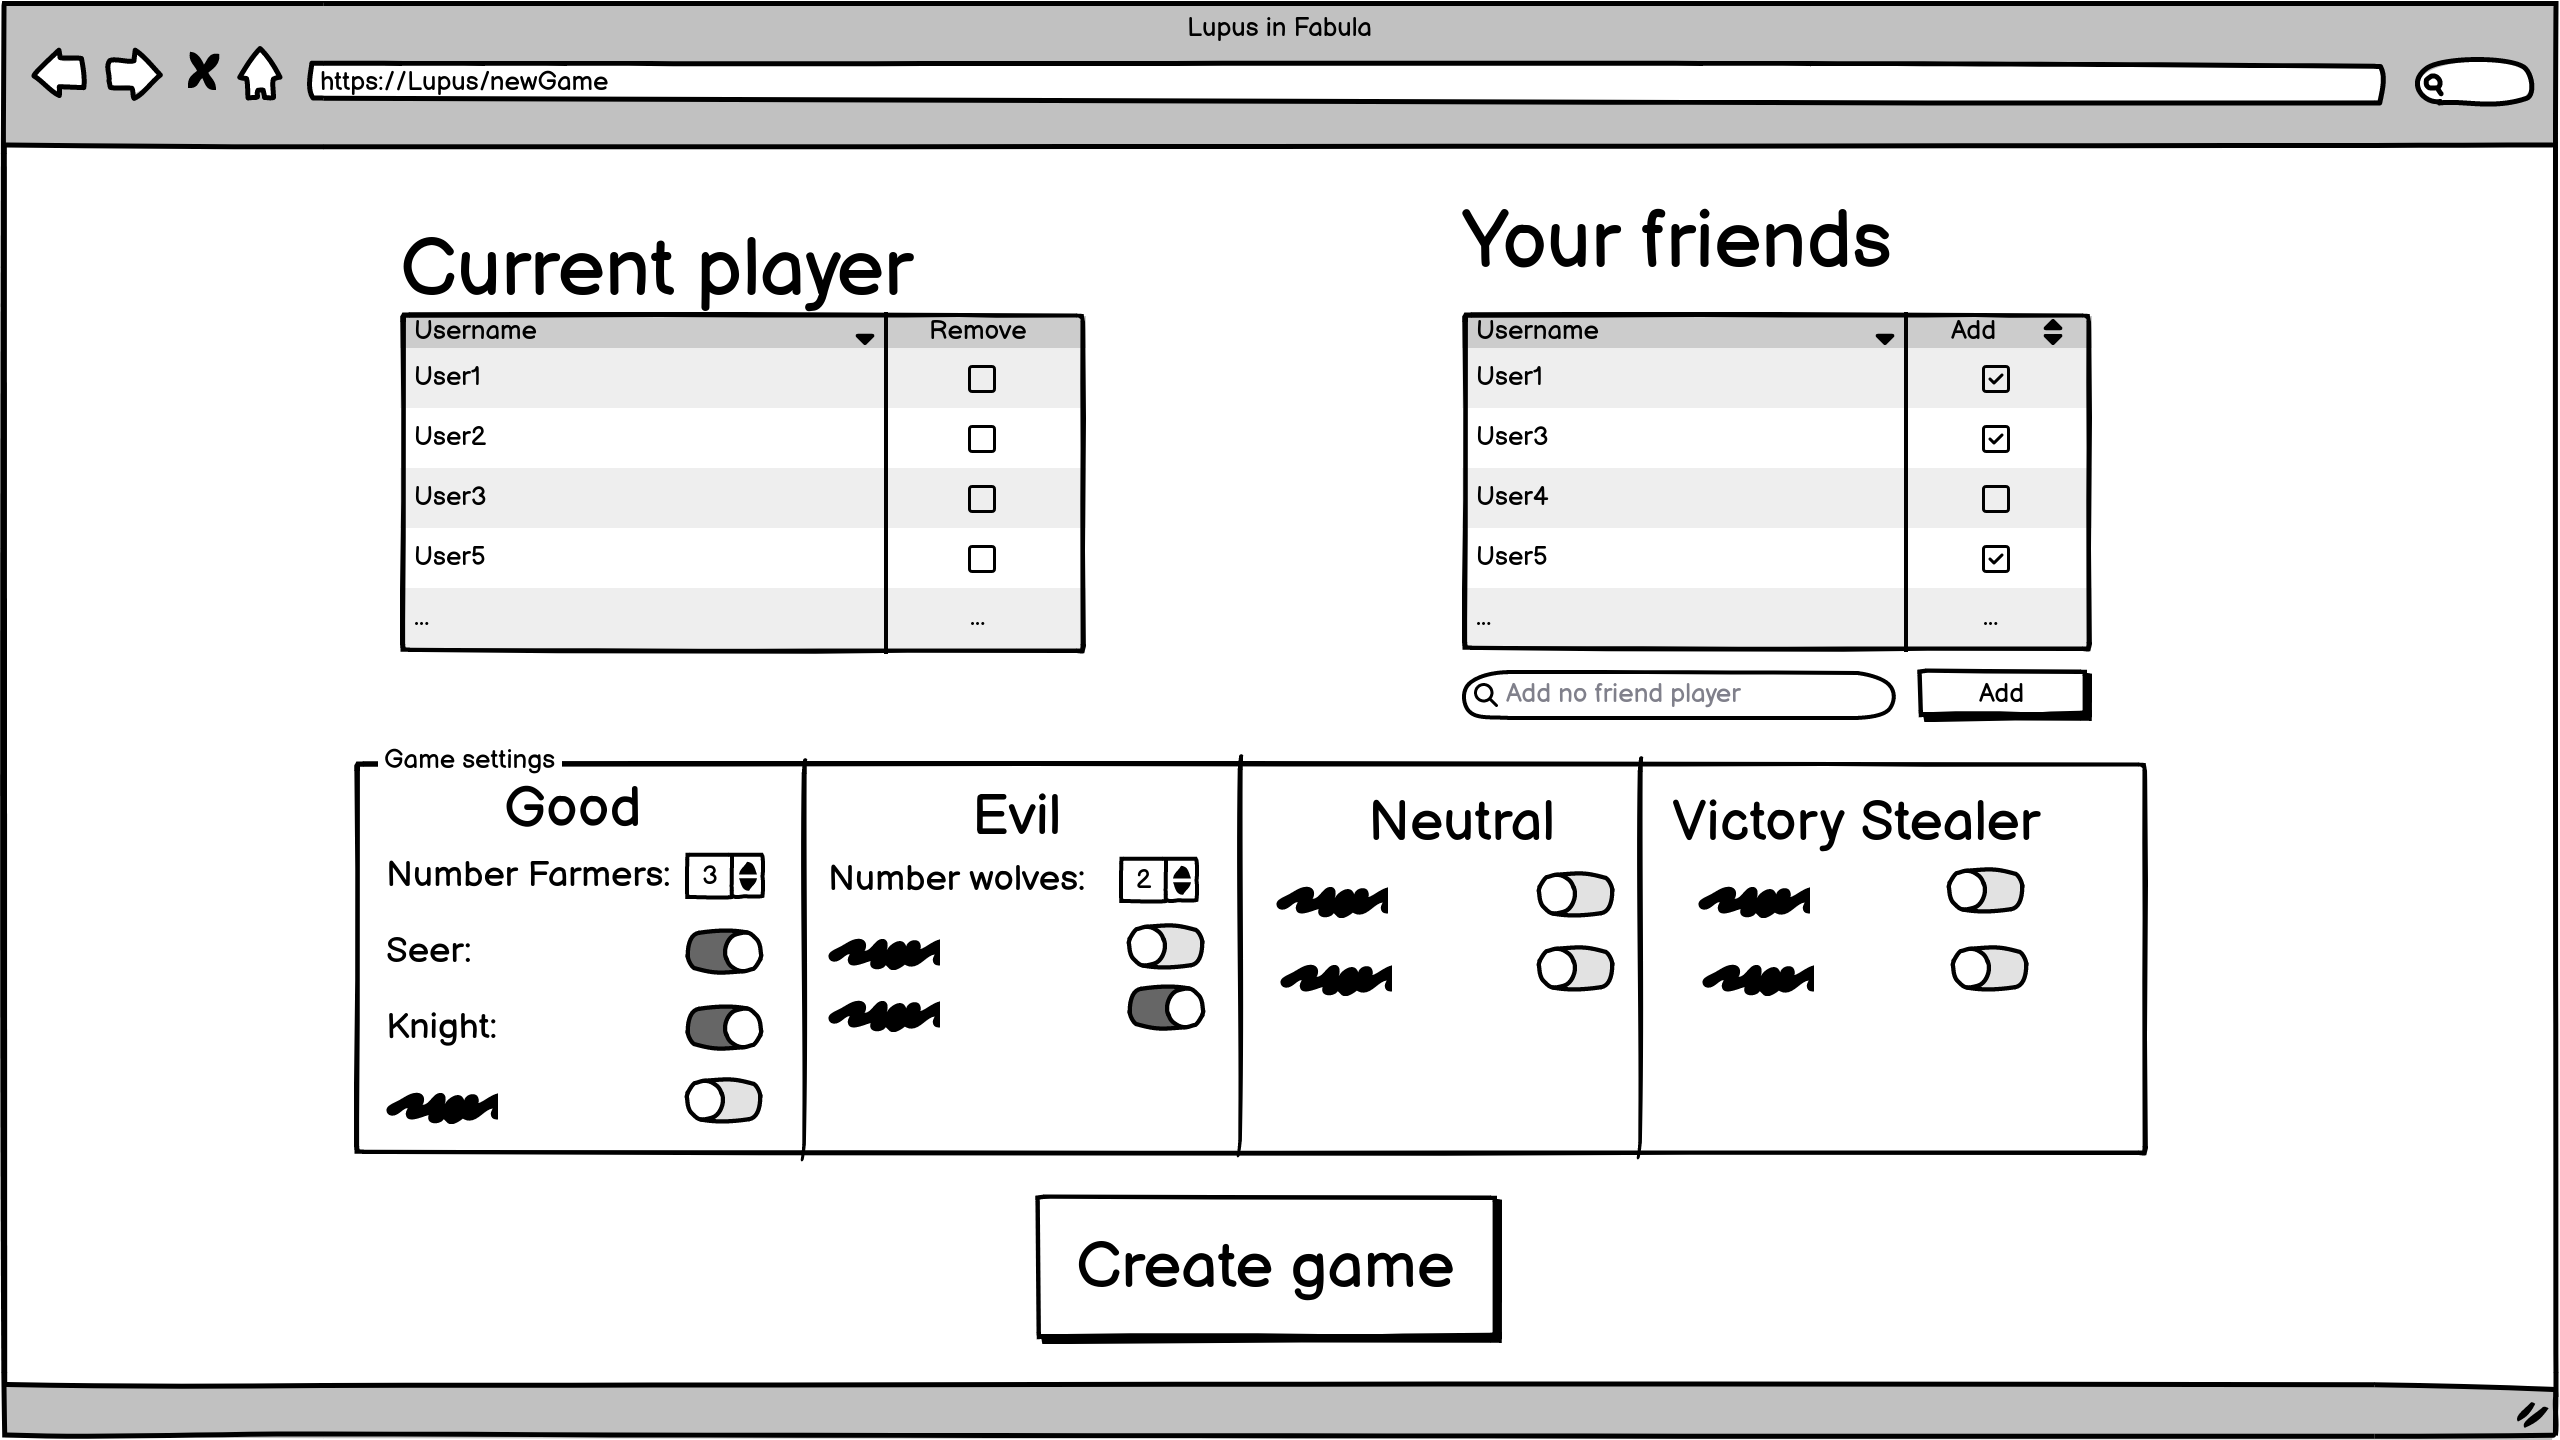
\includegraphics[height=6cm]{images/Page/GameCration.png}
    \caption{Game settings page}
    \label{fig:GameCration_page}
\end{figure}

From here the game-master has the possibility to create a new game, choose the game settings, such as how many wolves and how many farmers, and which other roles will be active. The Game-master can also choose the players who will play in that game, he can easily add his friends or search for them manually via username, (see figure \ref{fig:GameCration_page}).

\subsubsection{InGame Master view page (Interface Mockup)}
\begin{figure}[htb] 
    \centering
    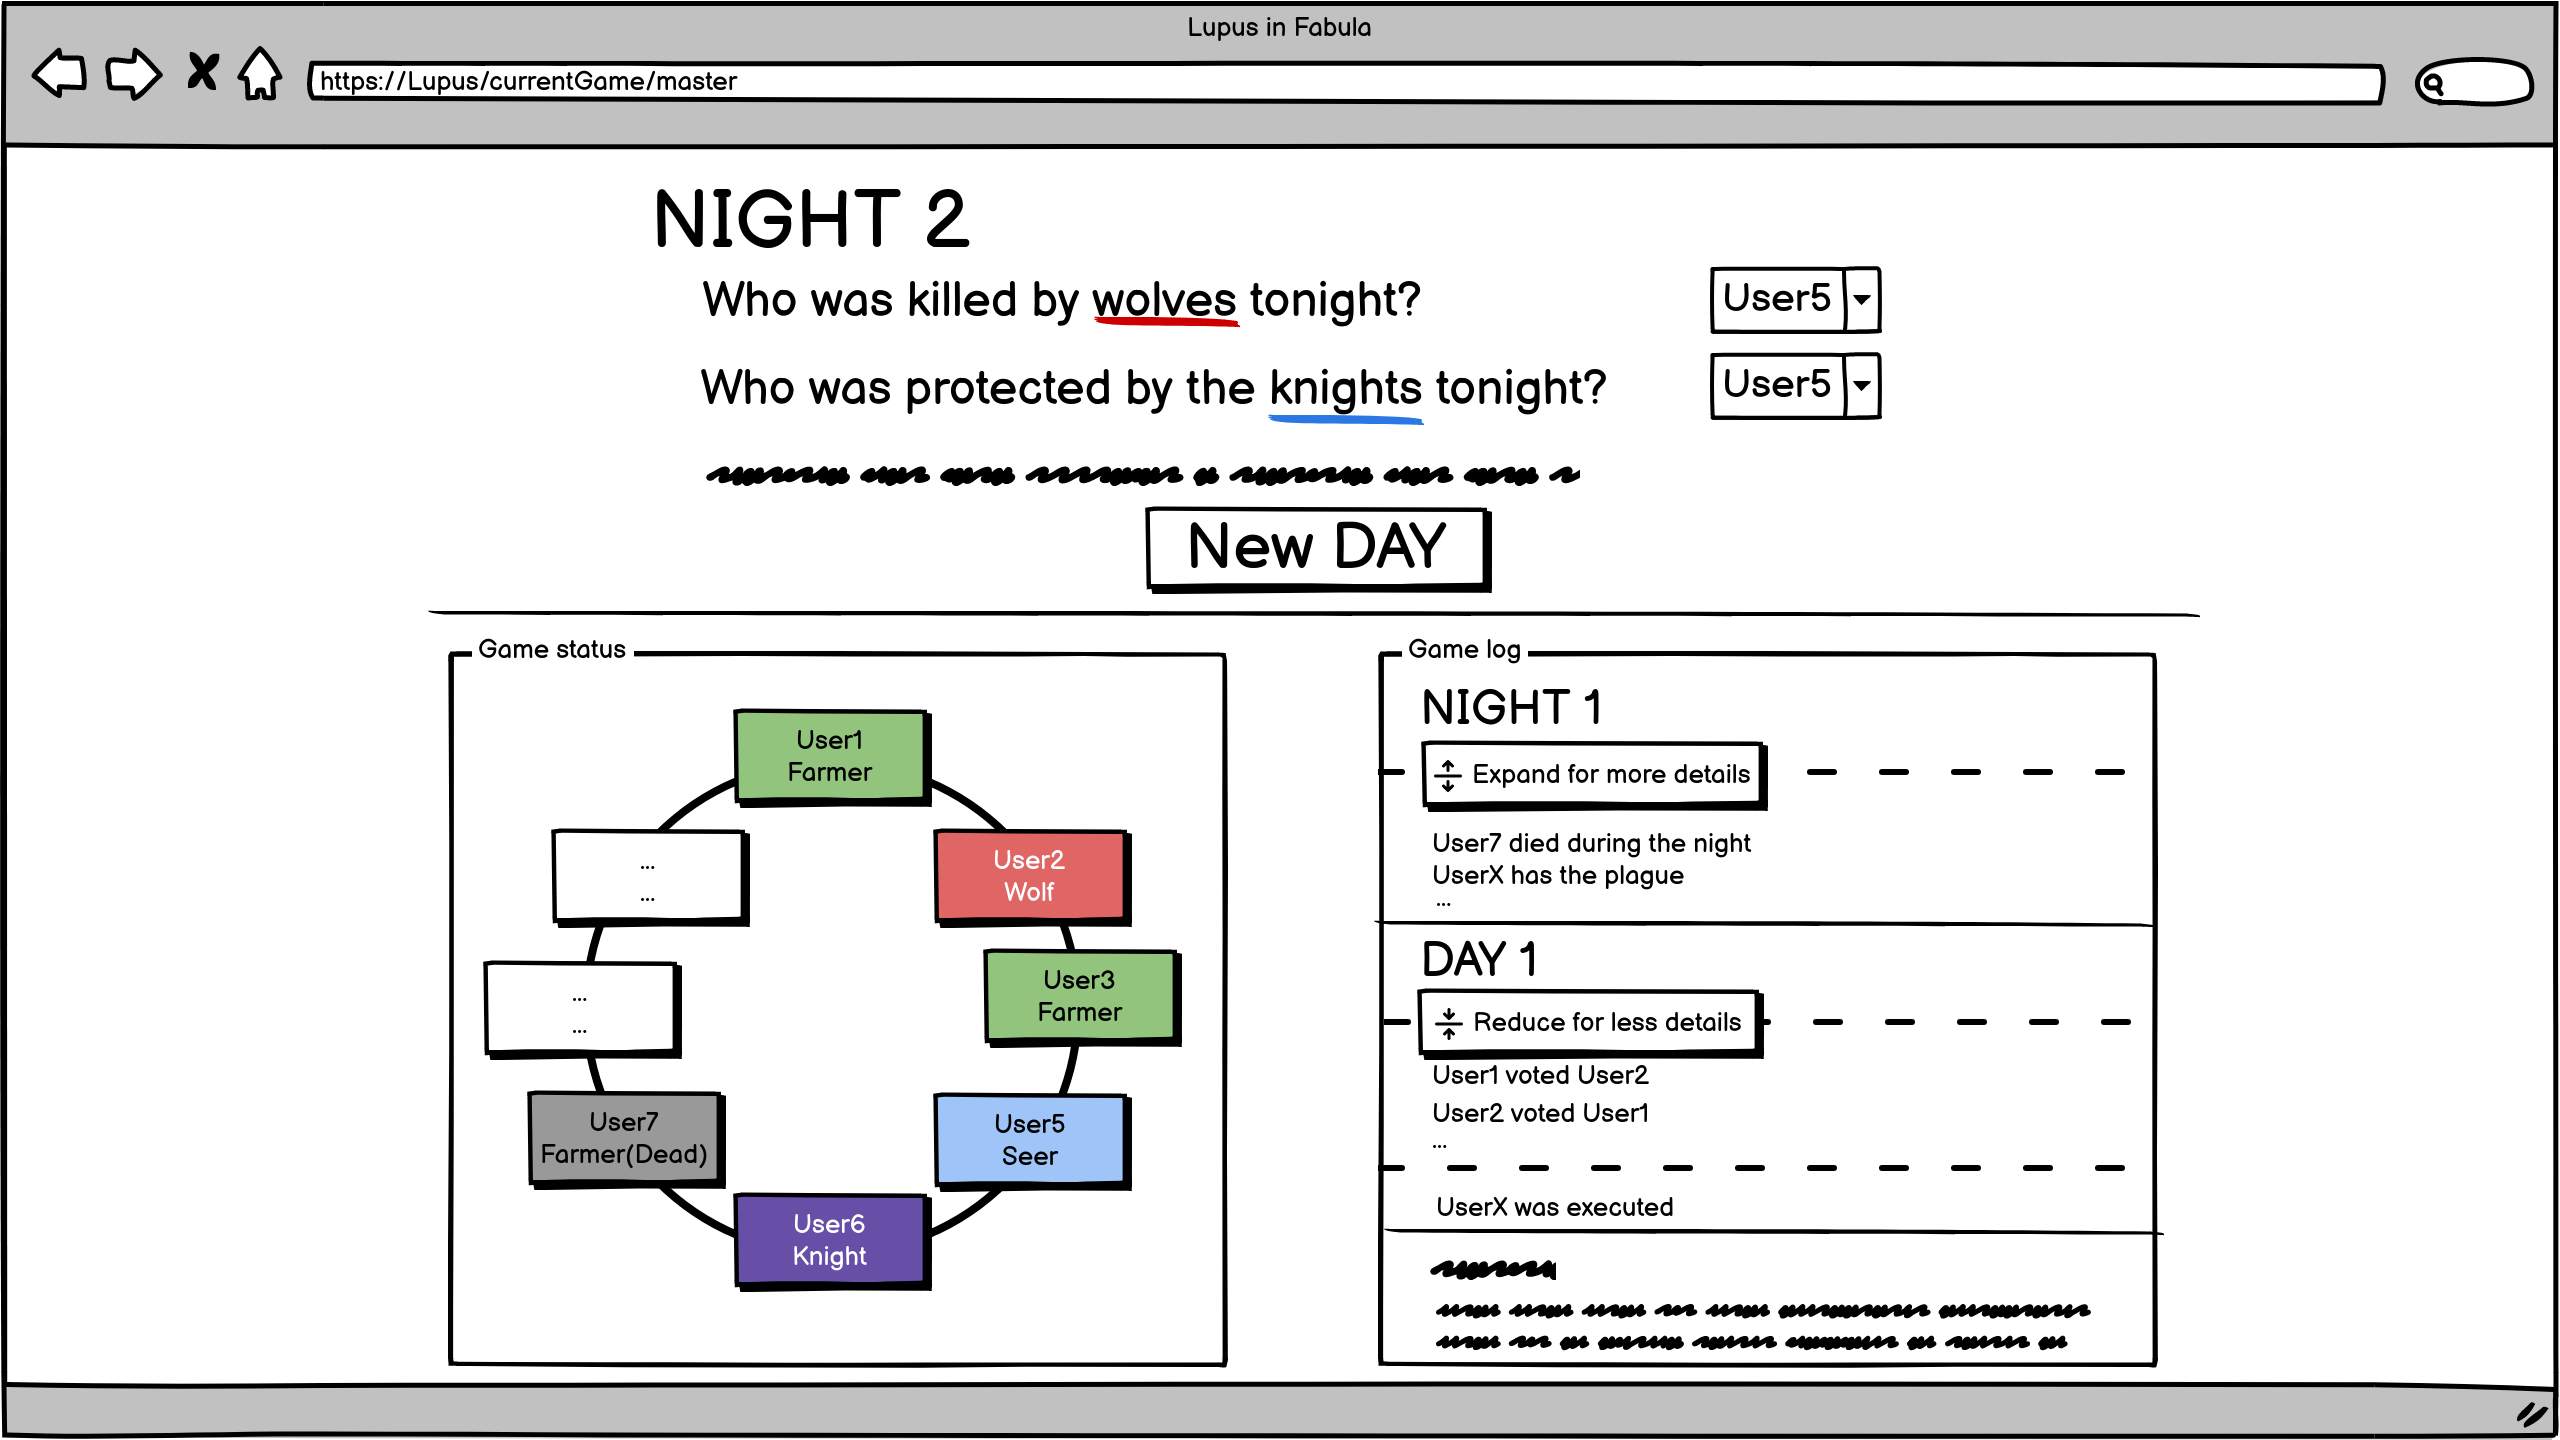
\includegraphics[height=6cm]{images/Page/Gamemaster.png}
    \caption{InGame Master view page}
    \label{fig:Gamemaster_page}
\end{figure}

From this page the Game-master is able to see the situation of the game, entering what happened during that phase, (visible in the top section of the mockup). During the night phase he is asked to select which player was eaten by wolves, which player was protected by the Knight, etc., while during the day phase he is asked which person each player voted to kill. At the end of each phase, (night or day), the application will respond what happened i.e. who died or who received some malus for example from the Plague Spreader.\\
The Game-master can see the current state of the game, so he knows the role of each player, whether he is alive or dead, (left section of the mockup). In addition he can see what happened in the previous phases via the logs (bottom right part of the mockup), so he can go through each phase to view what happened, (see figure \ref{fig:Gamemaster_page}).


\subsubsection{InGame Player view page (Interface Mockup)}
\begin{figure}[htb] 
    \centering
    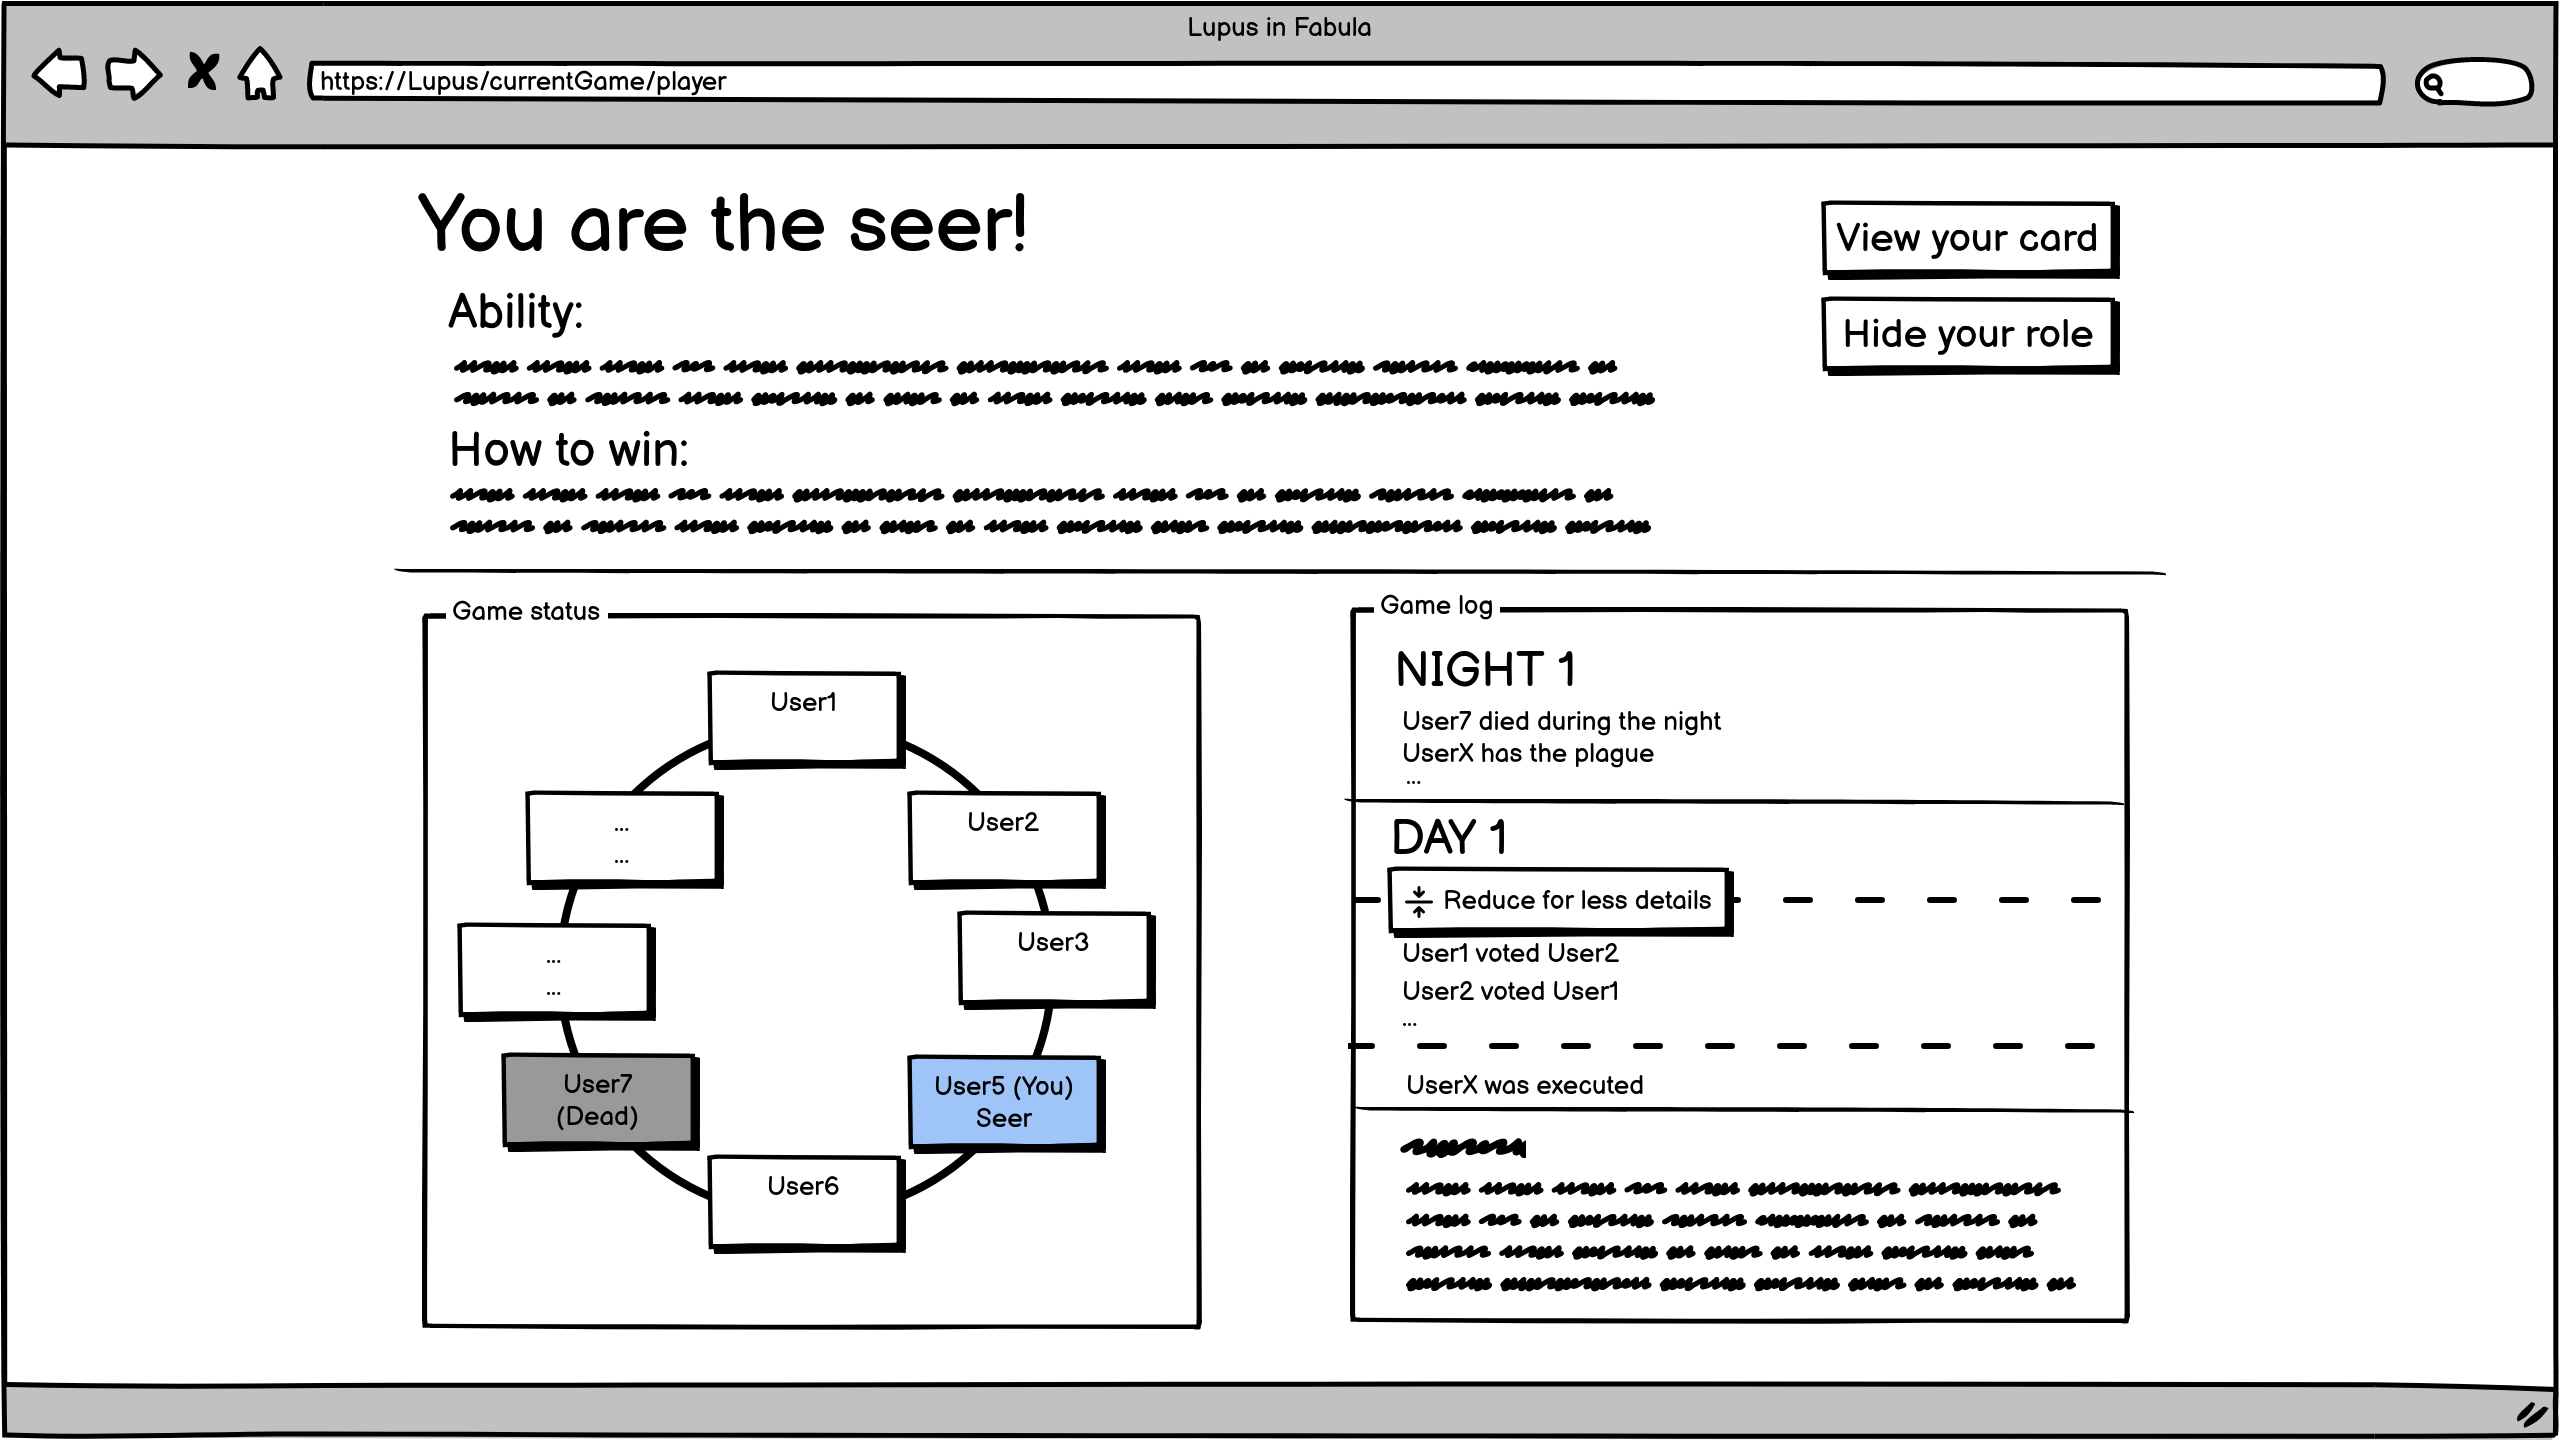
\includegraphics[height=6cm]{images/Page/Game player.png}
    \caption{InGame Player view page}
    \label{fig:GamePlayer_page}
\end{figure}


It is similar to the Game-master page, but with the difference that the player can only see his private game information, such as what role he has, seeing his card with the role description, and he can see the public information, i.e. who is still alive, who has died and who has been plagued by the Plague Spreader.\\
It can also see the match logs, but only the public information, so who died and in what round and phase and who voted who, (see figure \ref{fig:GamePlayer_page}).

\subsubsection{Log page (Interface Mockup)}
\begin{figure}[htb] 
    \centering
    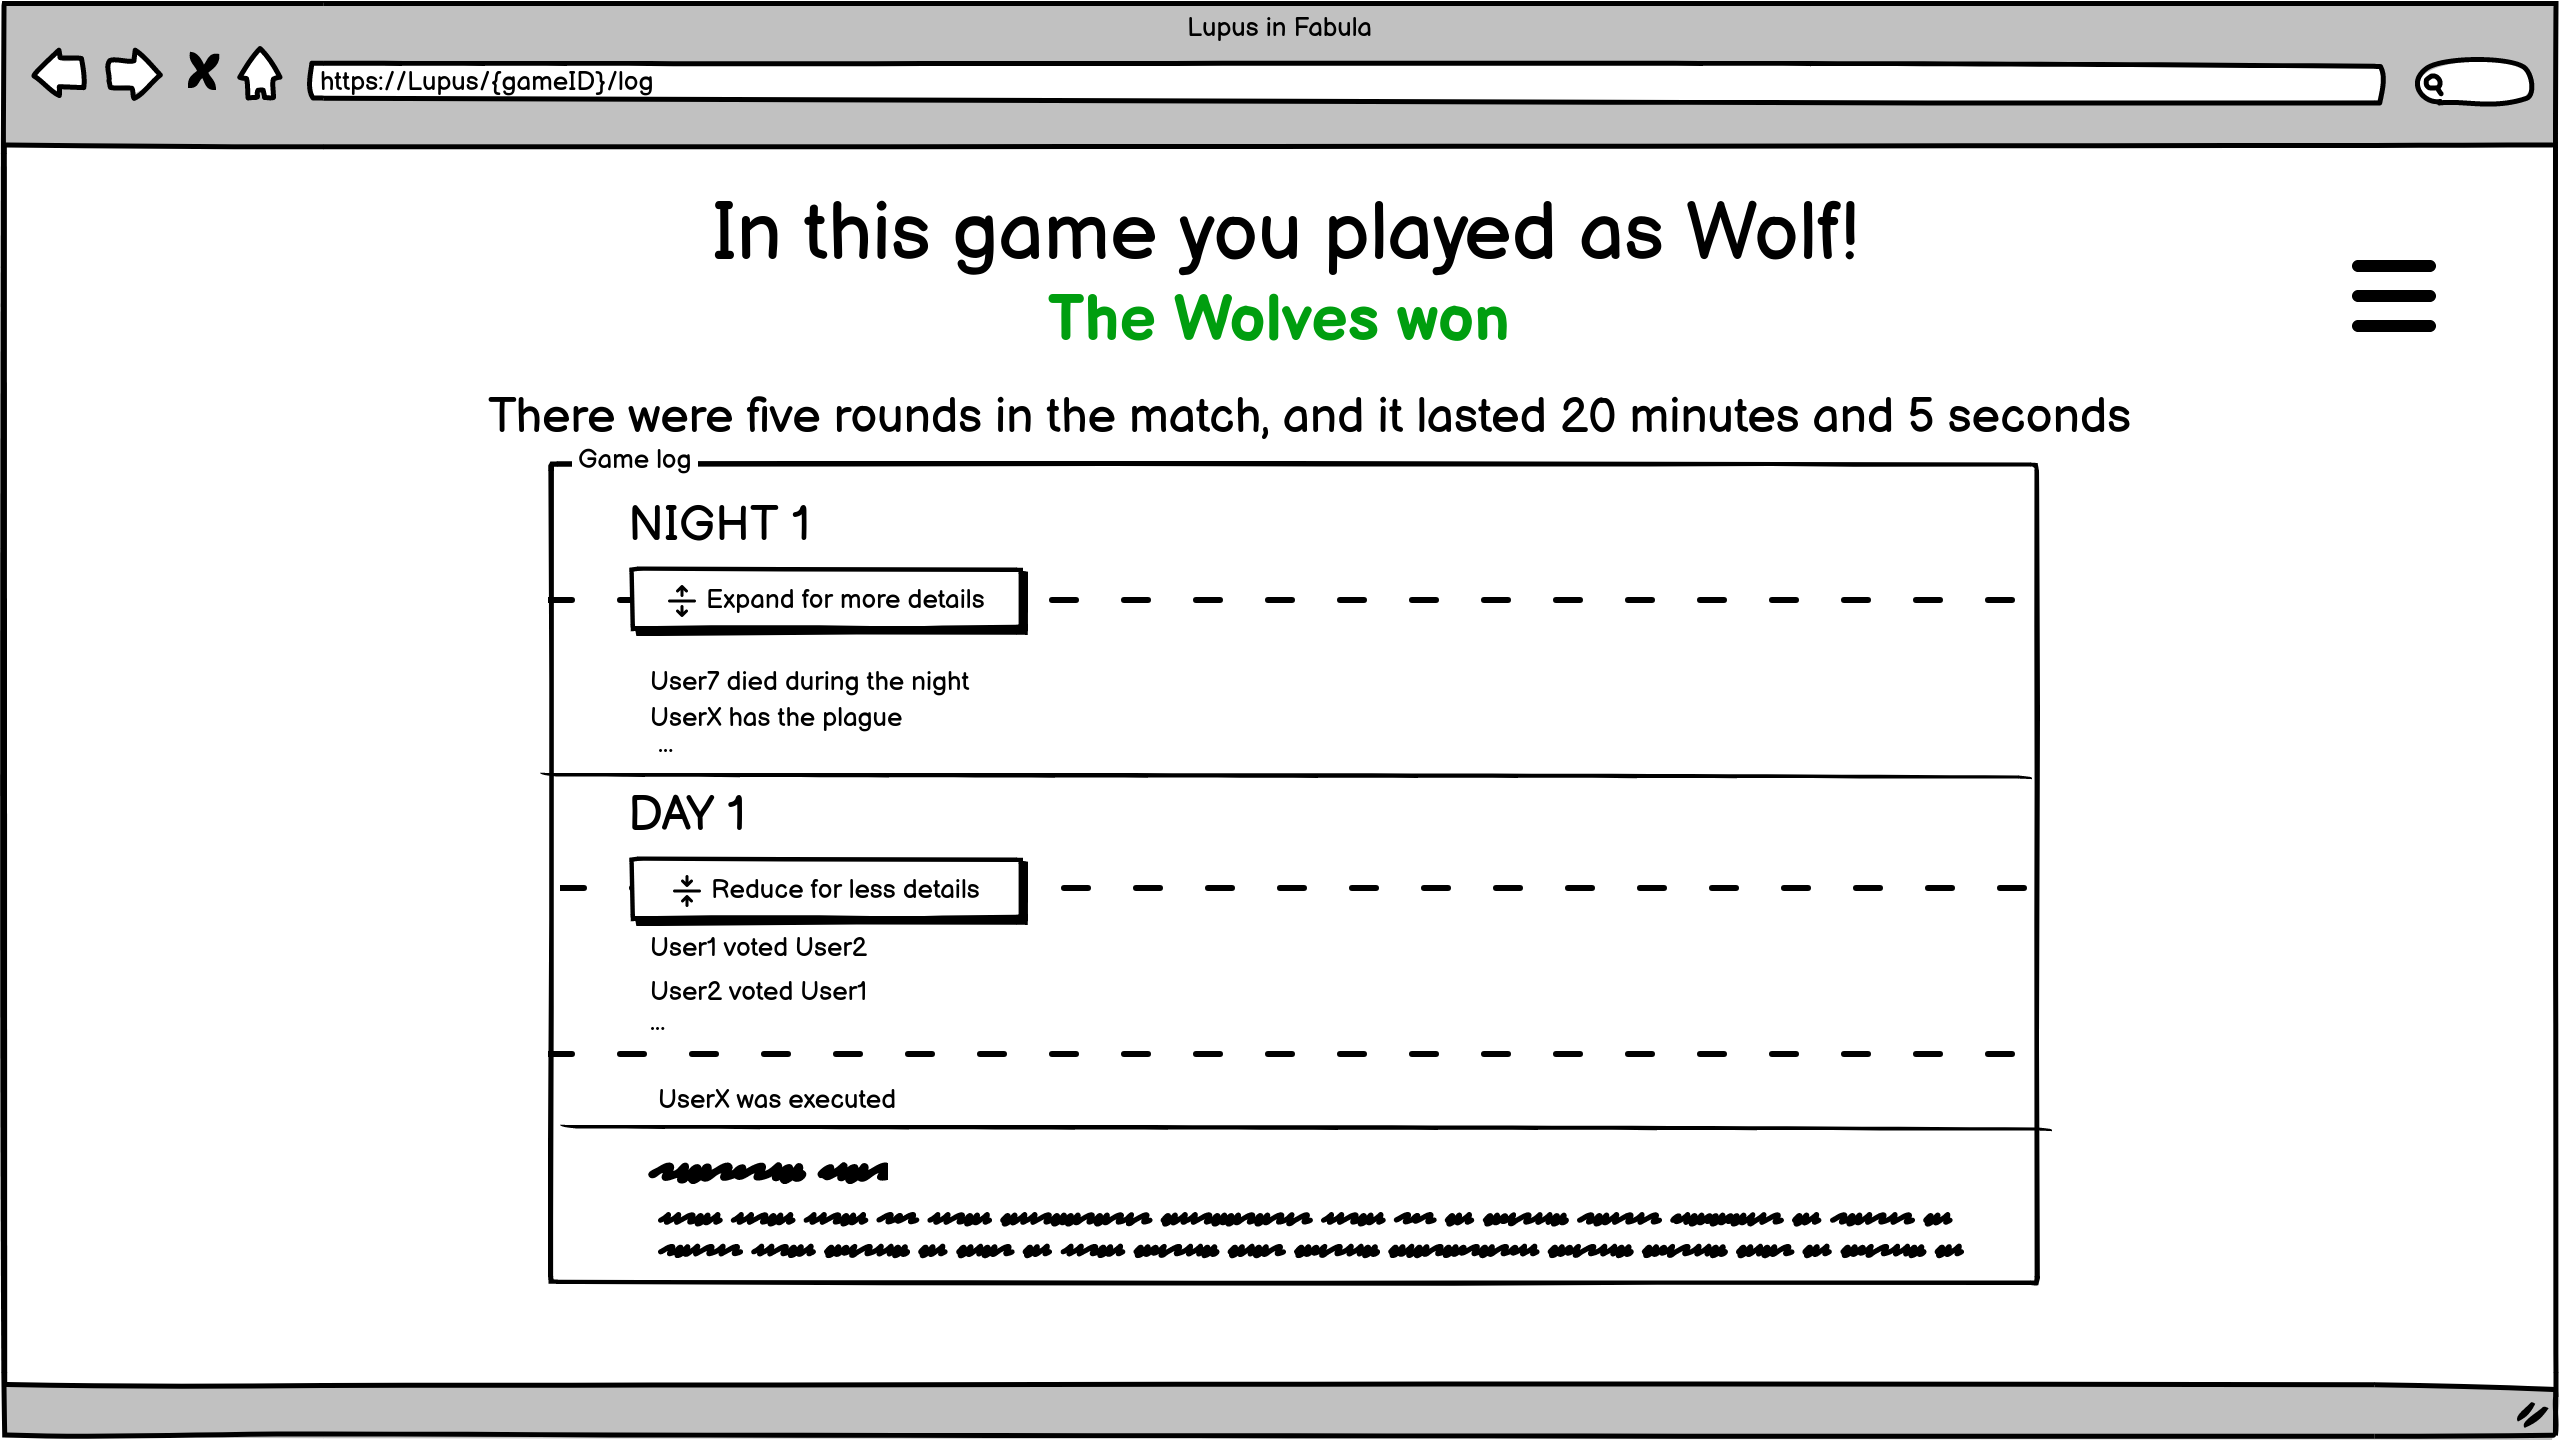
\includegraphics[height=6cm]{images/Page/Log.png}
    \caption{Log page}
    \label{fig:log_page}
\end{figure}

From here it is possible to see the logs of a game, i.e. what happened, who killed/protected/voted for whom, at what stage who died, who won etc.
This page shows all the information, even what happened during the night, but only when the game is over, if not it shows only the public information, (see figure \ref{fig:log_page}).

\subsection{Player section}

\subsubsection{User page (Interface Mockup)}
\begin{figure}[htb] 
    \centering
    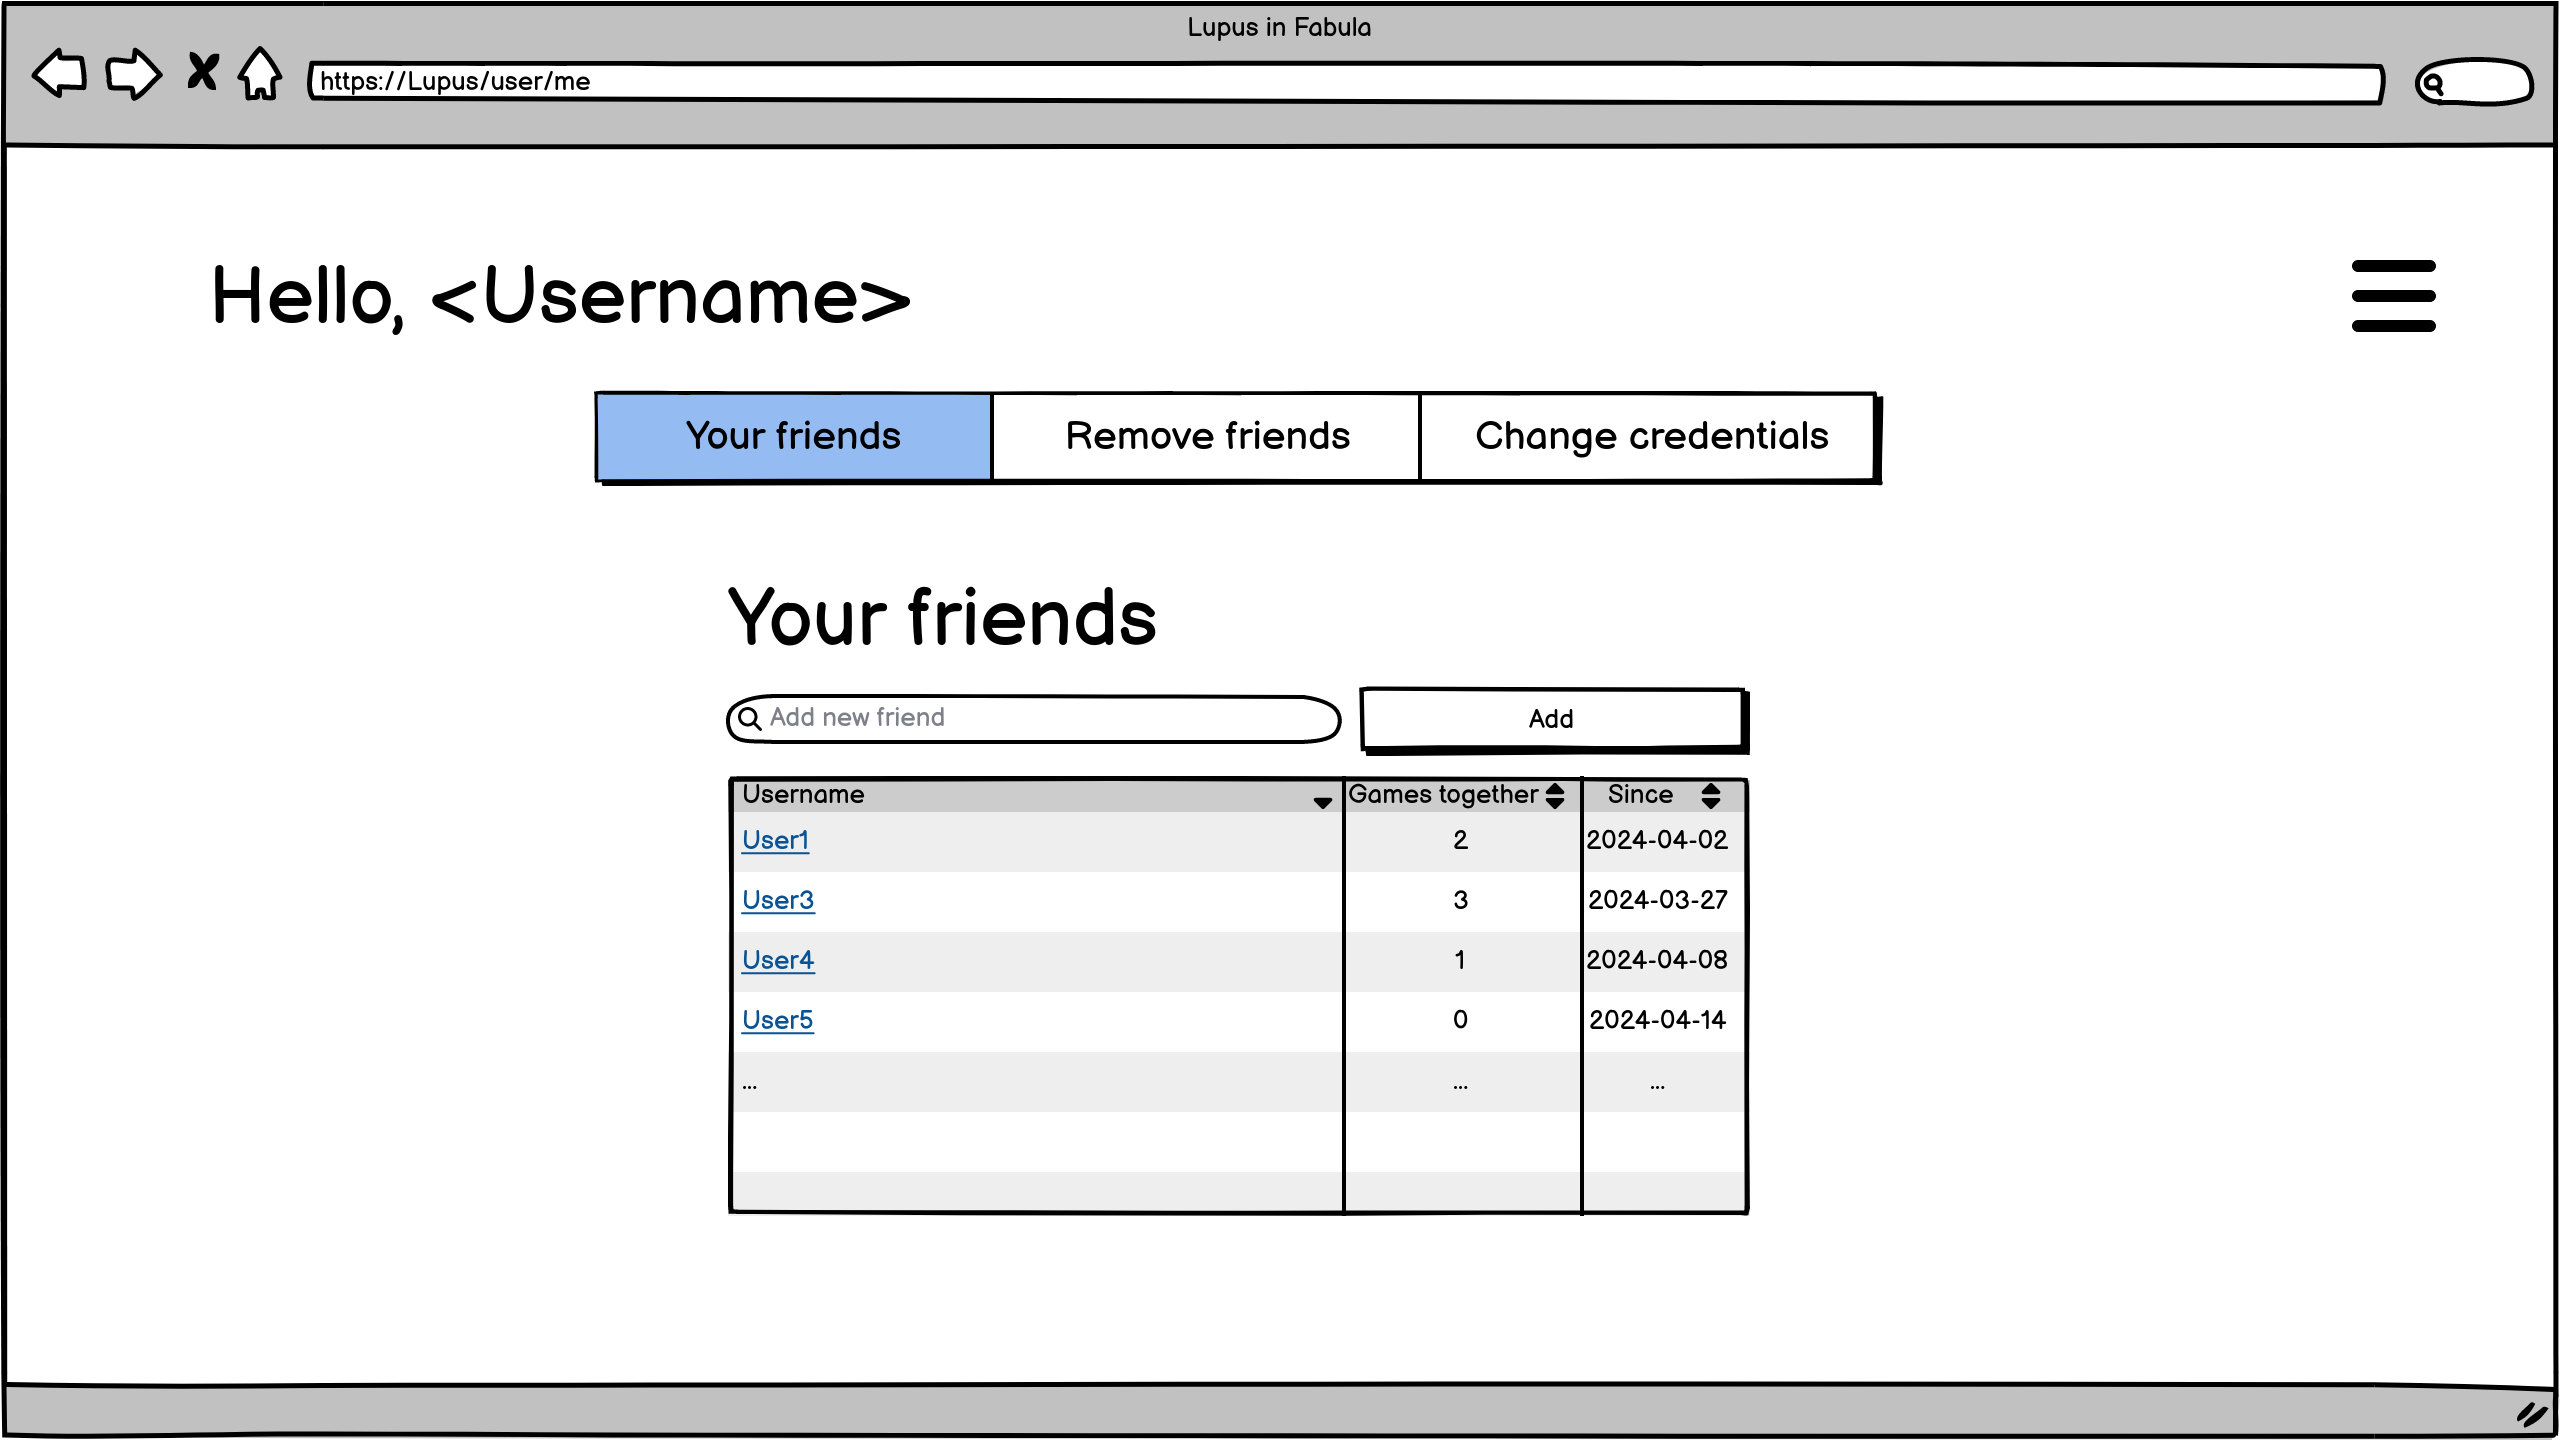
\includegraphics[height=6cm]{images/Page/User.png}
    \caption{User page}
    \label{fig:user_page}
\end{figure}

From this page, the user can manage his profile. He has the possibility of viewing his friends with some associated statistics, e.g. number of games played together and how long they have been friends. 
The user has the possibility of removing friends. Moreover, he can change his credentials, (email and password), (see figure \ref{fig:user_page}).

\subsubsection{Statistics and Logs page (Interface Mockup)}
\begin{figure}[htb] 
    \centering
    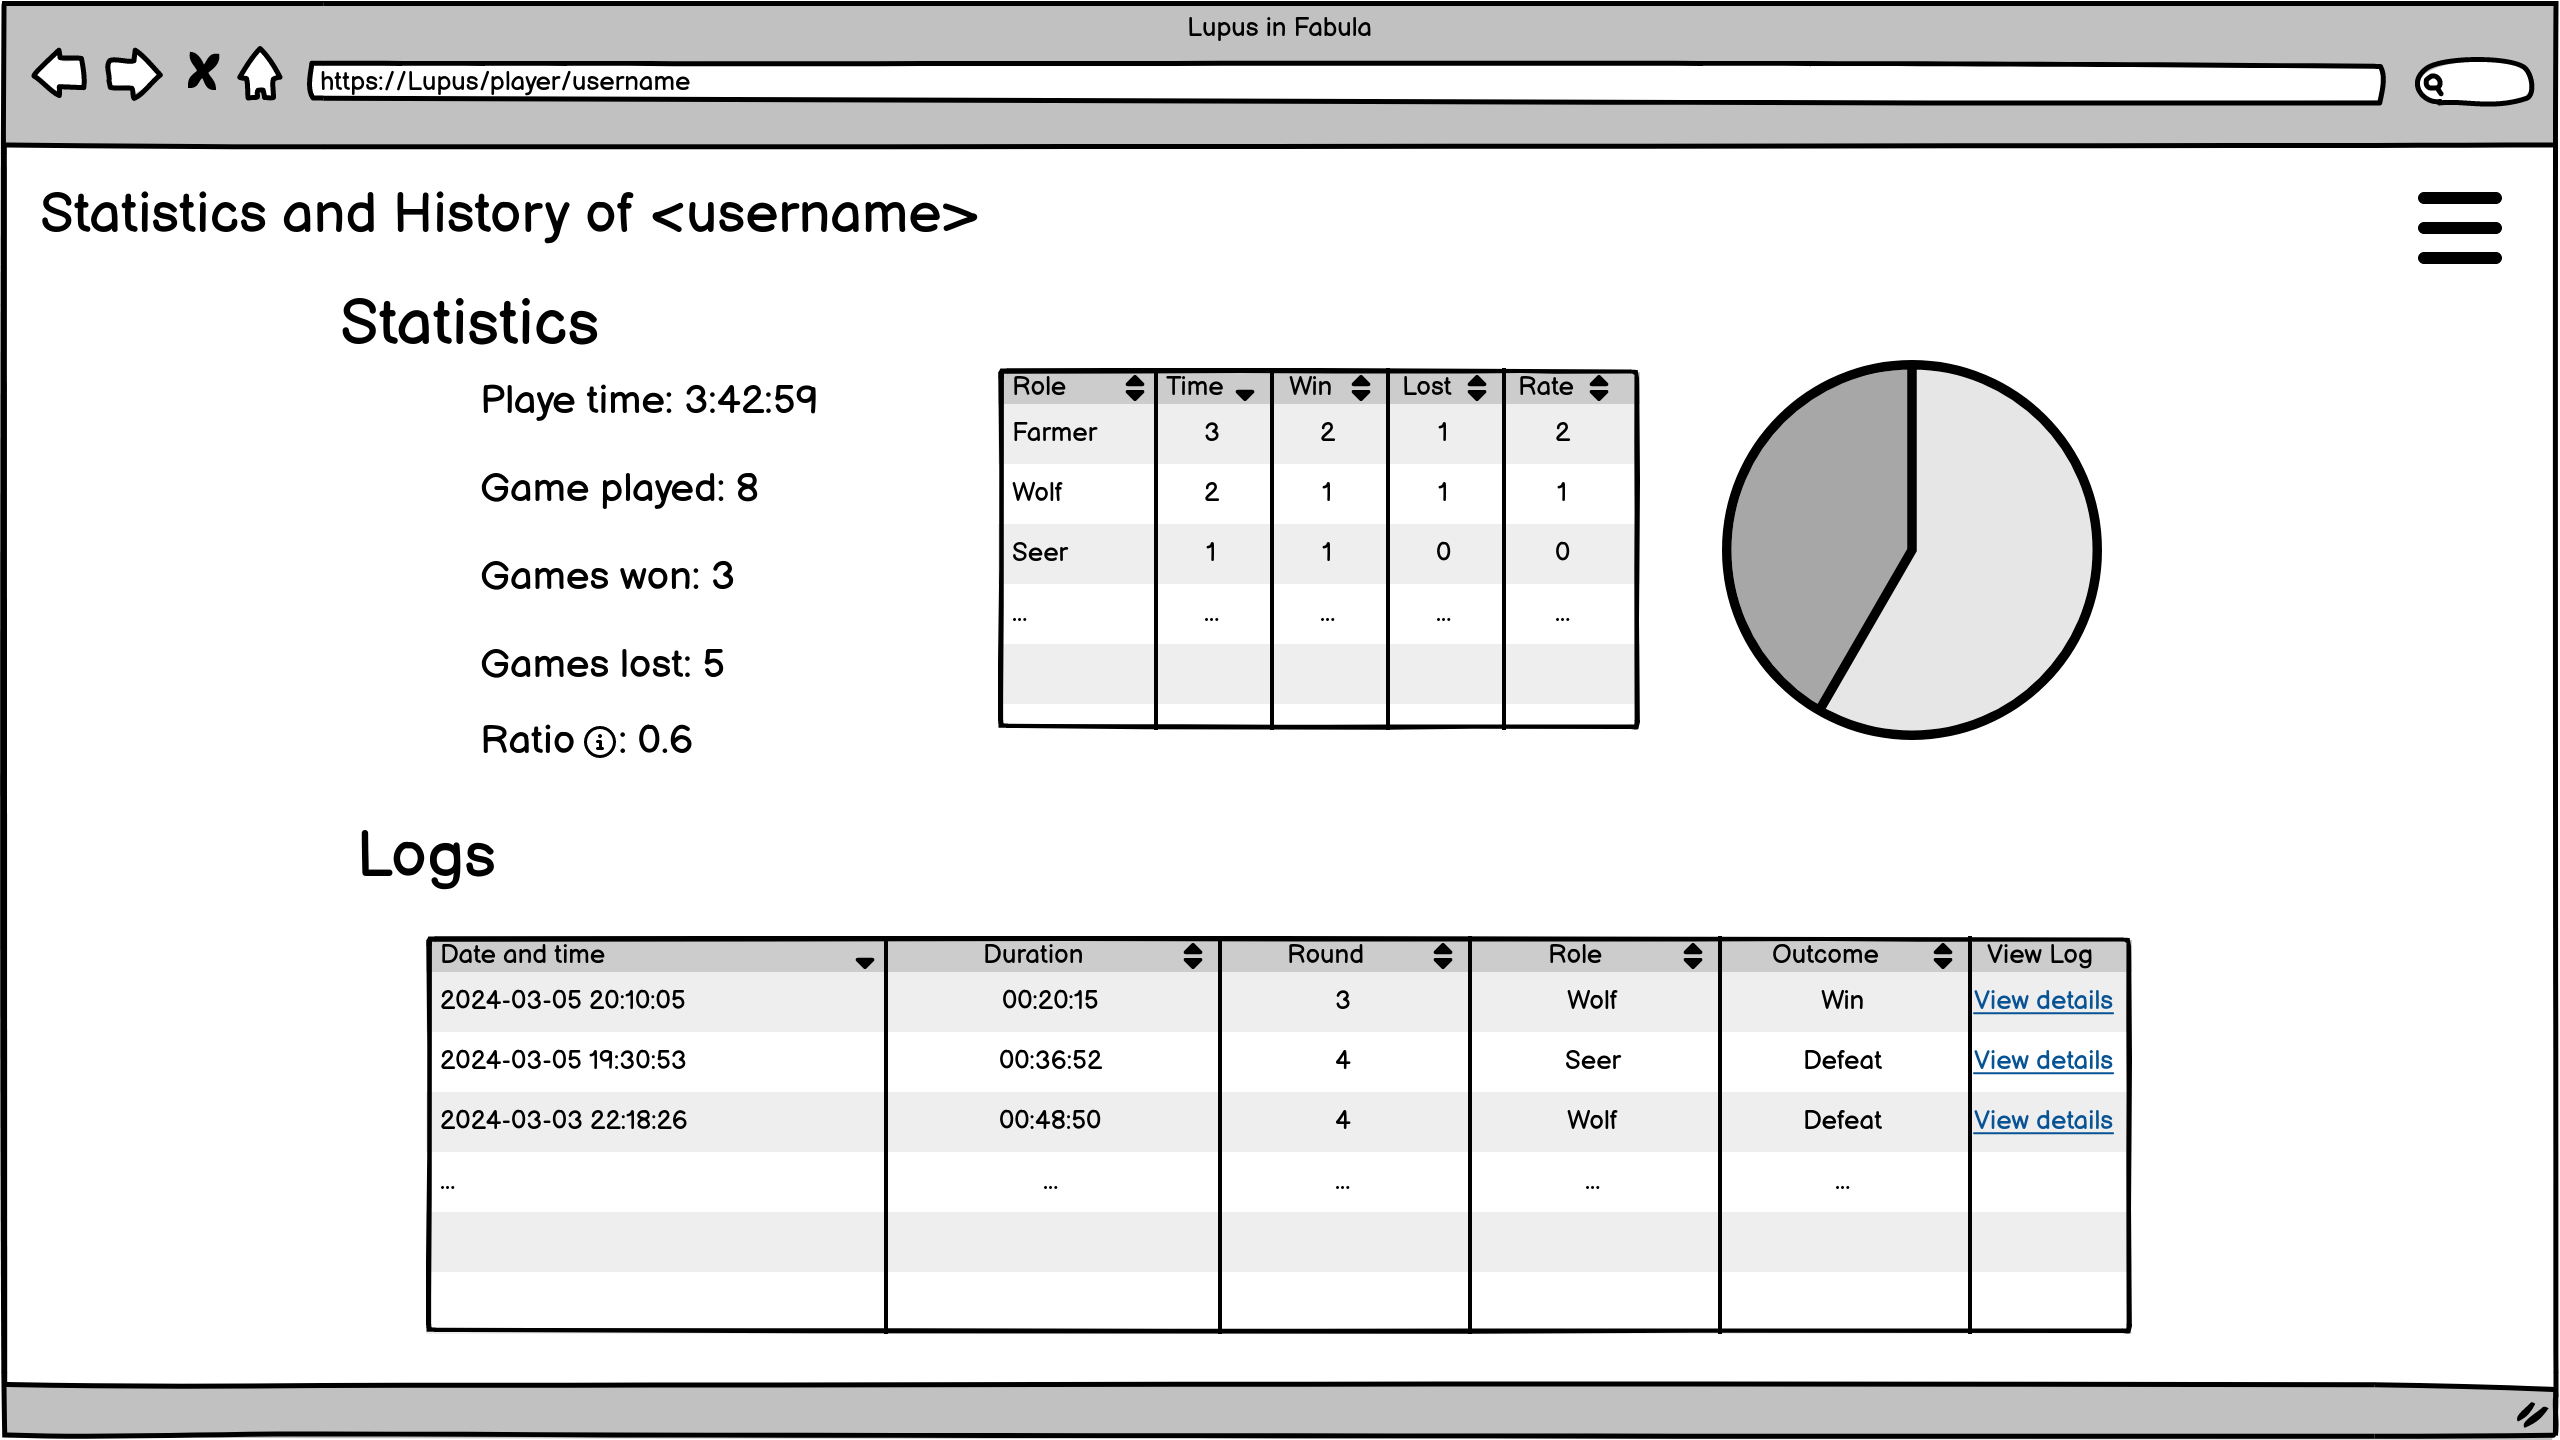
\includegraphics[height=6cm]{images/Page/Statistics.png}
    \caption{Statistics page}
    \label{fig:statistics_page}
\end{figure}

From here the user can see his statistics, i.e. the time played, the number of games played, won and lost, the roles he played and how many times. He can also see the history of the games he has played, with some associated information and has the possibility of viewing the entire match log, (see figure \ref{fig:statistics_page}).